\documentclass[10pt]{beamer}

\usetheme[progressbar=frametitle]{metropolis}
\usepackage{appendixnumberbeamer}
\metroset{sectionpage=none}


\usepackage{booktabs}
\usepackage[scale=2]{ccicons}

\usepackage{pgfplots}
\usepgfplotslibrary{dateplot,fillbetween}

\usepackage{xspace}
\newcommand{\themename}{\textbf{\textsc{metropolis}}\xspace}

\usepackage{tikz} 
\usetikzlibrary{arrows,shapes,tikzmark,decorations.pathreplacing,calc,fit,positioning,matrix,chains}

\usepackage{hyperref}
\usepackage{multimedia}

\usepackage{graphicx} % Load graphics
\usepackage{booktabs} % Nice tables
\usepackage{dcolumn} % Booktabs column spacing
\usepackage{threeparttable} % Align column caption, table, and notes
\usepackage{adjustbox} % Shrink stuff

\usepackage{multirow}
\usepackage{caption}
\usepackage{subcaption}
\usepackage{makecell}
%\usepackage{showframe} % Useful for debugging



% *****************************************************************
% Estout LaTeX wrapper
% *****************************************************************

%%Original code developed by Jörg Weber: see
%% https://www.jwe.cc/2012/03/stata-latex-tables-estout/
%% and
%% https://www.jwe.cc/blog/


\let\estinput=\input % define a new input command so that we can still flatten the document

\newcommand{\estwide}[3]{
		\vspace{.75ex}{
			%\textsymbols% Note the added command here
			\begin{tabular*}
			{\textwidth}{@{\hskip\tabcolsep\extracolsep\fill}l*{#2}{#3}}
			\toprule
			\estinput{#1}
			\\ \bottomrule          % 08 Dec 2021. Add these slashes.
			\addlinespace[.75ex]
			\end{tabular*}
			}
		}	

\newcommand{\estauto}[3]{
		\vspace{.75ex}{
			%\textsymbols% Note the added command here
			\begin{tabular}{l*{#2}{#3}}
			\toprule
			\estinput{#1}
			\\ \bottomrule          % 08 Dec 2021. Add these slashes.
			\addlinespace[.75ex]
			\end{tabular}
			}
		}

% Allow line breaks with \\ in specialcells
\newcommand{\specialcell}[2][c]{%
    \begin{tabular}[#1]{@{}c@{}}#2\end{tabular}
}

\newcommand{\sym}[1]{\rlap{#1}}% Thanks David Carlisle


%%%%%%%%%%% End of wrapper %%%%%%%%%%%%%%%%%%%%%



\title{Attention to Information about Social Out-groups}
%\subtitle{A modern beamer theme}
% \date{\today}
\date{May 12, 2022}
\author{Luisa Carrer}
% \institute{University of Zurich}
% \titlegraphic{\hfill\includegraphics[height=1.5cm]{logo.pdf}}

\begin{document}

\maketitle

\begin{frame}{Table of contents}
  \setbeamertemplate{section in toc}[sections numbered]
  \tableofcontents%[hideallsubsections]
\end{frame}

\section[Introduction]{Introduction}

\begin{frame}{Motivation}
\begin{itemize}
\item Perceptions of inequality that differ from reality (e.g. Alesina et al.(2021), Kraus et al. (2017))
\only<2->{\item High percentage of Americans' main source of news is TV} 
\only<4->{\item Newsroom employees are more likely to be white and male than U.S. workers overall (77\% vs 65\%)}
\end{itemize}
  \centering
  \only<3>{ 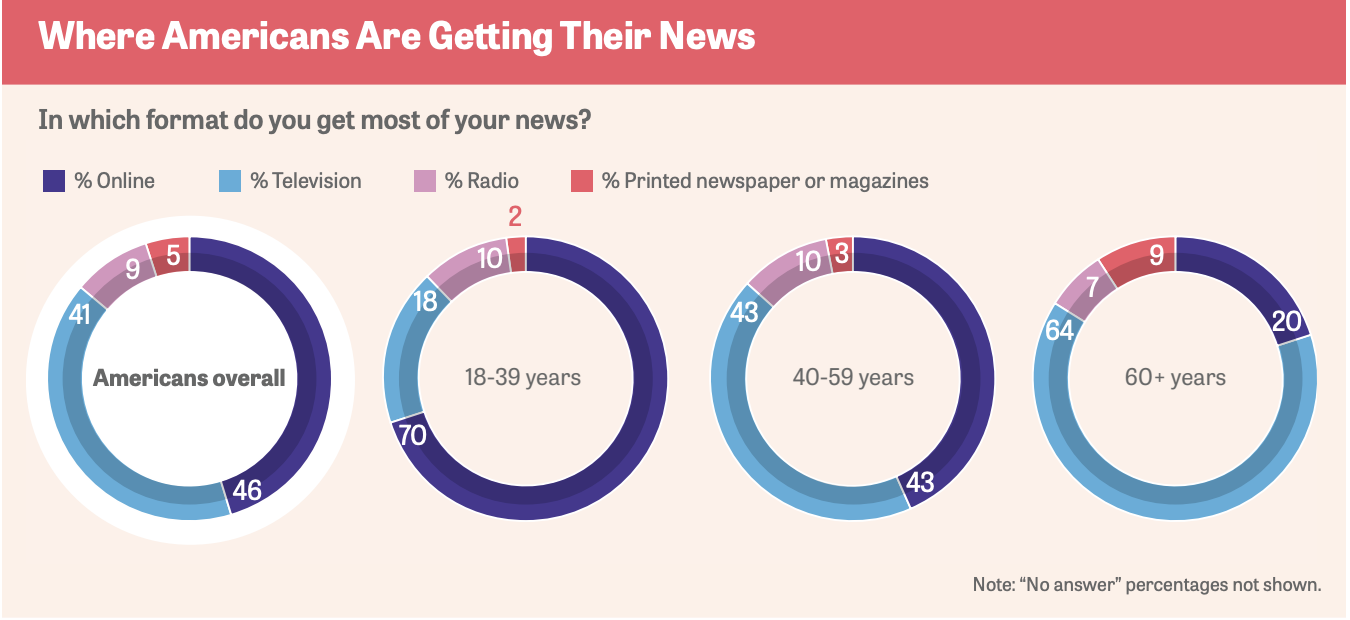
\includegraphics[width=1\textwidth]{news_source.png}}
  \only<5>{ 
  \begin{columns}
    \column{0.45\textwidth}
        \begin{center}
      \includegraphics[width=0.8\textwidth]{don_lemon cropped.jpg}
        \end{center}
    \column{0.45\textwidth}
        \begin{center}
        \includegraphics[width=0.8\textwidth]{bret_baier.jpeg}
        \end{center}
\end{columns}}
\end{frame}


\begin{frame}{Research Questions}
\begin{table}[!h]

\caption{Balance Table\label{tab:BT}}
\centering
\begin{threeparttable}
\begin{tabular}[t]{lrrrrrr}
\toprule
\multicolumn{1}{c}{ } & \multicolumn{2}{c}{\makecell[c]{Black\\Presenter} (N=798)} & \multicolumn{2}{c}{\makecell[c]{White\\Presenter} (N=797)} & \multicolumn{2}{c}{ } \\
\cmidrule(l{3pt}r{3pt}){2-3} \cmidrule(l{3pt}r{3pt}){4-5}
  & Mean & SD & Mean & SD & Mean Diff. & p-value\\
\midrule
Age & 40.463 & 12.647 & 40.044 & 12.470 & -0.417 & 0.514\\
Female & 0.474 & 0.500 & 0.478 & 0.500 & 0.004 & 0.862\\
Immigrant & 0.143 & 0.350 & 0.144 & 0.352 & 0.002 & 0.926\\
At least bachelor degree & 0.529 & 0.499 & 0.556 & 0.497 & 0.027 & 0.277\\
Employed & 0.642 & 0.480 & 0.636 & 0.481 & -0.005 & 0.824\\
Income in $\$\left[0,50\right]$ (th) & 0.371 & 0.483 & 0.364 & 0.481 & -0.007 & 0.768\\
Income in $\$\left[50,100\right]$ (th) & 0.305 & 0.460 & 0.340 & 0.474 & 0.035 & 0.130\\
Democrat & 0.538 & 0.499 & 0.511 & 0.500 & -0.027 & 0.281\\
Republican & 0.140 & 0.348 & 0.132 & 0.338 & -0.009 & 0.606\\
Voted in 2020 & 0.724 & 0.447 & 0.721 & 0.449 & -0.003 & 0.895\\
Hispanic & 0.078 & 0.268 & 0.097 & 0.296 & 0.019 & 0.181\\
Self-reported cheating & 0.068 & 0.251 & 0.075 & 0.264 & 0.008 & 0.553\\
\bottomrule
\end{tabular}
\begin{tablenotes}
\item \textit{Note: } 
\item * p $<$ 0.1, ** p $<$ 0.05, *** p $<$ 0.01. Test of equality of means calculated with standard errors corrected for block sampling.
\end{tablenotes}
\end{threeparttable}
\end{table}
\end{frame}


\end{document}


